\chapter{Installation}

The \frz is simply attached to the parallel bus. The parallel bus differs
between Atari XL and XE computers. In Atari XL computers the parallel bus
consists of the Parallel Bus Interface (PBI) which is labeled \fq{Parallel Bus}.
In Atari XE computers the parallel bus consists of the cartridge port and the
Enhanced Cartridge Interface (ECI) which are labeled \fq{Cartridge} and
\fq{Expansion}. The power supply of the \frz is taken from the parallel bus. In
Atari 600 XL and older Atari 800 XL computers the required power is available
directly on the parallel bus. It is no longer available there in new Atari 800
XL models and therefore has to be taken from the joystick port using the
power supply wire that is soldered to the freezer. Neither opening the Atari nor
soldering of any kind is required. Yet users with experience in soldering and with the
appropriate equipment have the option to add additional features.

The \frz consists of two parts, the freezer electronic in the black case and an
adapter board which establishes the connection to the PBI or ECI. The
adapter boards are available separately and hence provide a simple and cheap way
to use a \frz with Atari XL as well as with Atari XE computers.

\begin{figure}[h]
  \centering
  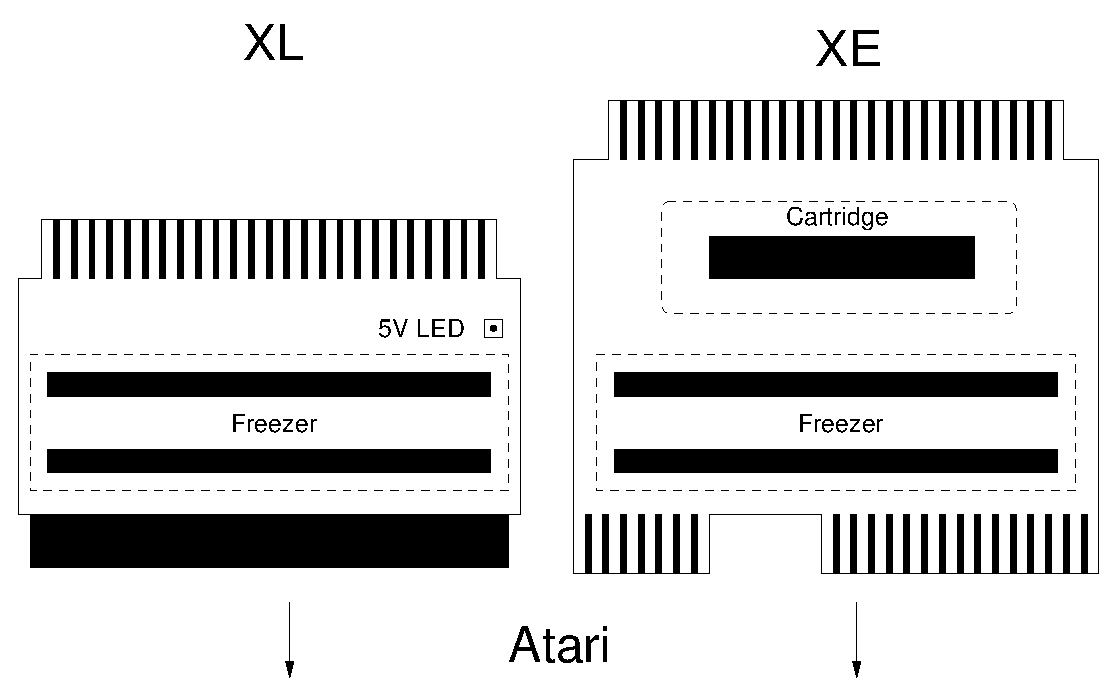
\includegraphics[width=35em]{adapter.eps}
  \caption{Atari XL and XE adapter boards}
\end{figure}

There is a small number of models from the XE series (mainly 65 XE) which do not
have an ECI port. These models only have a \fq{Cartridge} port and have no
\fq{Expansion} port. The freezer can unfortunately not be used with these XE
models. \newline

\textbf{Caution:} The freezer electronic and the adapter board are not connected
when they are shipped to prevent damage during transport. The Atari should
always be switched off to also prevent damage when attaching or detaching the
adapter board to/from the Atari or when attaching or detaching the freezer
electronic module to/from the adapter board.

\section{Verifying the power supply}
\label{sec:pbi5v}

Owners of Atari XL computer should verify the availability of the 5V power
supply on the PBI before assembling the freezer. Owners of Atari XE computer can
skip to the next step.

First switch the Atari off. Then attach the empty Atari XL adapter board without
the freezer electronic module to the PBI. Now switch the Atari on. If the 5V LED
on the adapter board lights up, then the 5V power supply is available on the PBI
and the power supply wire to the joystick port is not required. Even so, the
external power supply wire should not be cut off, but rolled up and put away
because it may be required for use on a different Atari without the PBI power
present. After that, switch the Atari off again and detach the adapter board
from the PBI.

\section{Assembling the freezer}

\subsection{Protecting from electro-static discharge}

You should \textbf{electrically ground} yourself before assembling the freezer
to discharge electro-static potentials which may be caused for example by the
carpet, shoes, clothing and so on. These potentials can reach several 1000 volts
and might destroy the XILINX chip and other ICs of the freezer. \textbf{Also
never touch the multi-pin connectors of the freezer without being grounded.}
This is true in general for all kinds of electronic parts. And though the Atari
is not too sensitive in this regard, it may still get damaged.

You best touch the heating or the protective earthing conductor pin of a power
outlet. Well suited, and very common in the professional area, are ESD
(electro-static discharge) wristbands to ground you permanently.

\subsection{Connecting the freezer electronic with the adapter board}

At the bottom of the module with the freezer electronic there are two multi-pin
connectors with 2x25 pins each. On the adapter board there are two female
connectors with 2x25 pins each. The freezer module with the freezer electronic
must be plugged into the adapter board in a way that the front side with the
switches points towards the PBI or ECI port of the Atari.
\textbf{The module must never be plugged in the other way around because that
may destroy the freezer.}

At first the module with  the freezer electronic must be positioned over the
female connectors in a way that all pins of the multi-pin connectors are located
over the corresponding female connectors. \textbf{No pins must overlap.} The
best way is to hold the module with the electronic in one hand and the adapter
board in the other hand.
Then place the module carefully on the board but do not press it and check from
all sides that the pins are aligned correctly. Now connect the module with the
adapter board using firm pressure. This works best if you turn the freezer
upside down. Use the fingers of both hands to hold the module on the left and
right side and then press the adapter board firmly in from the bottom with your
thumbs.

After plugging the module in you should verify that all pins are completely
inserted in the female connectors. If there are pins overlapping on one side,
the module with the freezer electronic must be unplugged and must be plugged
in again with correct alignment. If the pins are not completely inserted into
the female connectors you should firmly press until no part of the pins can be
seen anymore.

\subsection{Disconnecting the freezer electronic from the adapter board}

First the Atari must be switched off and the freezer must be detached from the
PBI or ECI port. The freezer electronic and the adapter board are quite
tightly connected via the 50 pin connectors. \textbf{You must never use too much
force or perform abrupt moves} otherwise the pins may break and the freezer can
be destroyed.

The following procedure works best: Lift the freezer module with the thumb by
pushing the left and the right edge of the freezer module in the middle between the
two multi-pin connectors. Lift it step by step carefully by $0.5$ up to at most
1 mm on one side and then on the other side. Make sure to pull out the contacts
equally on the left and right edge as well as in the front and the back row.

After about 2~mm the female connectors lose their grip. Now you have to
proceed with special precaution because otherwise the pins will be bent easily.
After about 5~mm you are done and the freezer electronic is disconnected from
the adapter board.

\section{Plugging the freezer in}

\subsection{Atari 600 XL (at least 64k RAM) and Atari 800 XL}

Remove the snapped in PBI plastic cover, bend the metal shielding carefully away
a little bit with your fingers and attach the freezer without using force.

\begin{wrapfigure}{r}{8em}
\centering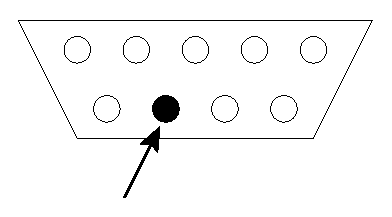
\includegraphics[width=8em]{joyport.eps}
\end{wrapfigure}
If the PBI
has a 5V power supply (see section \ref{sec:pbi5v}), the connection to the
joystick port can be omitted. If the power supply is not available on the PBI,
the power supply wire must be connected to pin 7 of the joystick port 2. Pin 7
is marked in the figure on the right.\newline

\textbf{Caution:} The power supply wire must never be disconnected while the
Atari is switched on, otherwise the Atari and/or the freezer can be damaged. If
the power supply wire is disconnected accidentally, the Atari must be switched
off immediately.

\subsection{Atari 800 XE, 65 XE and 130 XE}

Attach the freezer to the cartridge port and the ECI port at the back of
the Atari.


\section{Turning the freezer on}

\subsection{Setting the basic configuration}
\label{sec:baseconfig}

Turn all freezer switches to the left to activate the following basic
configuration:
\begin{itemize*}
\item \fsw{CartEmu}: \fval{OFF}, cartridge emulation off
\item \fsw{FlashWrite}: \fval{OFF}, write enable for flash ROM off
\item \fsw{OldOS}: \fval{OFF}, Oldrunner off
\item \fsw{Stereo}: \fval{OFF}, stereo POKEY mode off (not present)
\item \fsw{Ramdisk}: \fval{OFF}, 512k RAM extension off
\end{itemize*}

\begin{figure}[h]
  \centering
  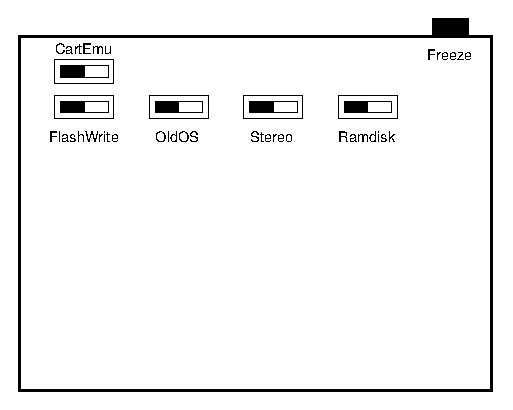
\includegraphics[width=22em]{freezer2011.eps}
  \caption{Switches on the \frz}
\end{figure}

\subsection{Activating the freezer}

Switch the Atari computer on and leave all other hardware switched off. If the
\fmsg{READY} message of the BASIC does not appear after the usual short delay,
but other suspicious symptoms occur (system crash, black screen, smoke), switch
the system off immediately and look for the problem. If the Oldrunner is active,
the message \fmsg{ATARI COMPUTER - MEMO PAD} is displayed instead of the \fmsg{READY}
message. If the cartridge emulation is active, the green screen with the
\fmsg{TURBO CARTRIDGE} menu of the cartridge emulation is displayed. In these
cases verify that you have really setup the basic configuration according to
section \ref{sec:baseconfig}.

If \fmsg{READY} is displayed, simply press the \fsw{Freeze} button on the
upper right to display the freezer main menu. If nothing happens, the freezer is
attached poorly, the power supply wire (if present) is not connected correctly
or the freezer broke down. By pressing the \fkey{SPACE} key you can return from
the freezer main menu to the BASIC. Now verify if BASIC reacts to keyboard
input. If this is not the case, then there is a problem. If everything worked
fine up to this point the freezer is ready.

If the freezer does not work correctly for any reason, send a letter or e-mail
with the description of the symptoms first before sending the freezer back.
Because of the 100\% final assembly tests of every freezer it is practically
impossible that the problem is due to the freezer. Most likely the assembly or
the Atari itself are the cause for the problem. It is better to rule out these
possible reasons before sending the freezer back for verification. This prevents
unnecessary delays and costs.

\subsection{Creating the system disk}

Right after the successful installation of the \frz a system disk should be
created. The system disk contains the flash program for writing to the flash ROM
from the Atari and the freezer software. With this disk the \frz can be reset
at any time to its state at delivery. In the state at delivery the flash ROM
contains the software required for creating the system disk as follows:

\begin{enumerate}
\item Switch the Atari off and connect a disk drive.
\item Turn the \fsw{CartEmu} switch right to activate the cartridge emulation.
\item After switching the Atari on the menu of the cartridge emulation should
appear.
\item Press \fkey{D} to load the default settings and confirm them with \fkey{RETURN}.
\item Now you are in the \fq{\frz System Disk Writer} software. Insert an empty
disk in the disk drive \fq{D1:} and press \fkey{RETURN}. The software now
formats the disk in medium density and writes the freezer software.
If an error occurs (\eg due to a disk defect), the message \fmsg{ERROR} is
displayed and you have to insert a new disk and restart the program. To this
end simply confirm the \fmsg{restart program?} prompt with \fkey{Y}.
To be on the safe side, a second copy of the system disk should be created.
Write protect this second copy and store it in a safe location.
\item After creating the system disk successfully, switch the Atari off and turn
the\linebreak
\fsw{CartEmu} switch back (to the left) again to its original position.
\end{enumerate}

If anything goes wrong and you lose the system disk or overwrite it
accidentally (yes, things like that can happen sometimes), there still is the
option to download an ATR disk image of the system disk from the internet at
\url{http://turbofreezer.horus.com}.

\subsection{Activating the stereo POKEY mode (optional)}

If the Atari has a stereo POKEY extension that is in stereo mode, the
\fsw{Stereo} switch must be turned right. This way the freezer also saves the
hardware registers of the second POKEY in the shadow RAM. When the freezer is
activated, the second POKEY is disabled. When the program is resumed, its
correct previous state is restored again.

The general rule is that the position of the switch must correspond exactly to
the configuration of the Atari. Changing the switch position during operation is
allowed, but then the shadow RAM will contain wrong information. To fix this you
have to press \fkey{RESET} to trigger a re-initialization of the custom chip
area by the operating system. Alternatively change the switch position only when the
Atari is switched off.

\subsection{Activating the integrated 512k RAM extension (optional)}

As a special feature the freezer contains an integrated, battery backed 512k RAM
extension. With this every Atari can be extended easier than ever from 64k to a
total of 576k. And since the RAM extension is battery backed, the data in the
RAM extension remains intact also after switching the Atari off.

Turning the \fsw{Ramdisk} switch right activates the RAM extension. A possibly
present internal RAM extension in the Atari is automatically deactivated then.

\subsection{Using cartridges with the Atari XE}

Because the freezer occupies the cartridge port on Atari XE computers, there is
an additional cartridge port present on the XE adapter board. With this you can
continue to use cartridges even though the freezer is attached. The cartridges
have to be plugged in the adapter board with the label towards the Atari. Never
plug the cartridge in the wrong way, otherwise the cartridge, the freezer and
the Atari can be damaged.

There are cutouts around the cartridge port where a \fq{plastic tray}, like
those that are present in the cartridge port of Atari XL computers, can be
inserted. This relieves you from the tedious unlocking some cartridges require.
These \fq{plastic trays} are unfortunately not available separately. The only
way to obtain one is taking a defective Atari XL computer apart.

\section{Extended configurations for experts in soldering}

{\bfseries Warning: All of the following extensions are definitely only for
experts in soldering. If you are not such an expert strongly consider
finding one rather than trying this yourself. It is not worth ruining the poor
Atari or the freezer due to unhandiness.}

\subsection{Providing an internal power supply}
\label{sec:add5vpbi}

Whoever owns an Atari 800 XL without power supply on the PBI can add this
retroactively, but this is difficult and requires good skills. If you are not
confident enough you can simply prolong the power supply wire of the freezer to
the power supply inside the Atari. In both cases the joystick port remains free
for its actual purpose.

To discourage beginners, the following description of the modification is
limited to the absolute minimum. Experts will get along without problems. If you
found an \fq{expert} and realize that he is groping in the dark, then this is
the last chance to stop this obvious amateur.

You can tap the power supply at the end of L1 from where a conductor path leads
to the shielded part. The ferrite bead is located within spitting distance to
the power switch. To this spot you can either solder the prolonged power supply
wire of the freezer, or use two wires to connect the 5V power to pins 47 and 48 of the PBI.
These pins are the second to last pins before pin 49 and 50. One is one the
upper side of the board, one is on the lower side of the board. Soldering to the
lower side is much more difficult because the Atari must be disassembled
completely for this. In addition soldering to the ends of the mating surface
without having solder creeping to the active part of the  mating surface is
finicky. The latter must be prevented in any case.

\subsection{Installing a SYSTEM RESET key}
\label{sec:systemreset}

For using the Oldrunner and for freezing programs which do not use interrupts,
it is beneficial to install a \fkey{SYSTEM RESET} key which triggers a
non-maskable interrupt (NMI) that cannot be disabled. The key button is
installed such that pin 6 of the ANTIC can be switched to ground. It is best to
connect the key button to the corresponding pull-up resistor. You can tap the
pin at best at the pull-up resistor. In the Atari 800 XL and all Atari XE models
this resistor is R1. In the Atari 800 XL it is R34, and in the Atari 1200 XL it
is R7.

{\bfseries Warning: In addition to the general warning from the first section it
applies here that mechanical works are required to install the key button.
These works require additional tools and manual skills to achieve a good-looking
result.}

\subsection{Providing compatibility with 1MB RAM extensions}

The \frz uses the refresh line to stop the Atari. Unfortunately this leads to
compatibility problems with all internal RAM extensions that use an own refresh
logic based on the refresh signal of the ANTIC. This applies mainly to 1MB RAM
extensions such as the Newell RAM extension. Most of the 256k RAM
extensions and the extended memory of the Atari 130 XE are not affected.
The problem can be solved easily with two additional components. You require a
small signal Schottky diode, \eg of type \fq{BAT 85} and a 4.7kOhm resistor.

{\bfseries Warning: In addition to the general warning from the first section it
applies here that the pin of the ANTIC must be treated with special
precaution. The pin breaks very easily if it is bent too much.}

After opening the Atari pin 8 of the ANTIC must be bent up. The wire that
leads from pin 8 to the RAM extension must be unsoldered first. If the ANTIC is
socketed, pull the ANTIC out of the socket and bend the pin up carefully. It is
sufficient to bend the pin up only far enough that it stays outside of the
socket when the ANTIC is put back into the socket. If the ANTIC is soldered to
the board, cut the pin right above the board with a mini wire cutter and bend it
up carefully.

At first solder the diode between the bent up pin 8 and pin 8 of the socket (or
the Atari main board if there is no socket). The cathode (marked with a ring on
the housing) must be connected to the ANTIC; the anode must be connected to the
socket. The most simple solution for this is to solder the diode directly to pin 8
of the ANTIC and to solder a thin wire from the anode to the lower side of the
board and connect it there to pin 8.

One end of the resistor must be connected to the anode of the diode; the other
end of the resistor must be connected to pin 21 of the ANTIC (+5V). Now the
wire that was unsoldered from pin 8 of the ANTIC can be soldered again to pin 8
of the ANTIC.
